
%%%%%%%%%%%%%%%
%%%      CHAPTER      %%%
%%%%%%%%%%%%%%%

\chapter{{\EvoEvoSim}, a multi-scale model dedicated to Evolution of Evolution}
\label{ch:part2:methodology}

\paragraph{}
\paragraph{}
\paragraph{}
\paragraph{}
\paragraph{}
\paragraph{}
\paragraph{}
\begin{center}
\large \textbf{The development of {\EvoEvoSim} is part of the European project EvoEvo (FP7-ICT-610427). The description of work of the project and the deliverables related to {\EvoEvoSim} are freely available at \href{www.evoevo.eu}{www.evoevo.eu}.}
\end{center}

\newpage

%%%%%%%%%%%%%%%%%%%%%%%%% SECTION : INTRODUCTION %

\begin{quote}
Although there has been much discussion on what is the appropriate level on which Darwinian selection operates, we now know that in many cases the interesting features arise through the occurrence of multiple levels of selection which act in concordance and/or in conflict.\\
\citep{hogeweg-and-takeuchi-2003}
\end{quote}

\section{Meet {\EvoEvoSim}}
\label{sec:part2:methodology:intro}

\begin{figurehere}
\centerline{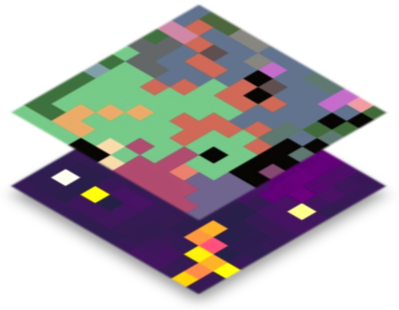
\includegraphics[width=0.2\textwidth]{part2_logo_evo2sim.png}}
\caption{{\EvoEvoSim} logo.}
\end{figurehere}

{\EvoEvoSim} is a \textbf{multi-scale} and \textbf{individual-based} model of evolution, inspired from \textbf{pearls-on-a-string} \citep{crombach-hogeweg-2008} and \textbf{sequence-of-nucleotides} \citep{beslon-et-al-2010a,hindre-et-al-2012}.
As discussed in introduction, developing complex representations of the genotype-to-phenotype map and fitness landscape has been a primary goal in the conception of this model. To do so, we used the \textbf{bag-of-tuples} formalism (also discussed in introduction) to develop an  \textbf{artificial chemistry} allowing for multi-level evolution. 

Two major objectives constrained the development of {\EvoEvoSim}: \textbf{(i)} integrate a maximum number of pertinent biological structures and levels (genome, genetic regulation, metabolic network, cell, population, ...) to enable deep exploration of EvoEvo, and \textbf{(ii)} maintain the model complexity low enough to enable its practical use. As such, a tough compromise had to be made between the degree of realism (the number of assumptions we want to pick to build the model, see \citealt{servedio-et-al-2014}), and what we want the model to tell us. This modeling problem is well-resumed by the concept of Medawar zone: as illustrated in Figure \ref{fig:part2:methodology:medawar_zone}, the Medawar zone is the area where the model complexity is most likely to produce fruitful results. Too simple models are unlikely to produce novel or significant results. Too complex models may not succeed at all or may be rejected by the research community at large \citep{loehle-1990}.
\begin{figure}[!ht]
\centering
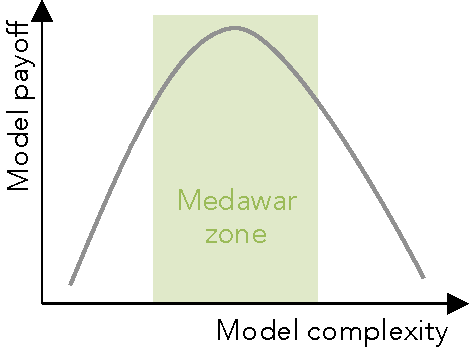
\includegraphics[width=0.4\textwidth]{part2_medawarzone.pdf}
\caption[The Medawar zone.]{\textbf{The Medawar zone.} The Medawar zone is the area where the model complexity is most likely to produce fruitful results. Too simple models are unlikely to produce novel or significant results. Too complex models may not succeed at all or may be rejected by the research community at large \citep{loehle-1990}.}
\label{fig:part2:methodology:medawar_zone}
\end{figure}

As described in the description of work of the EvoEvo project\footnote{Available at \href{www.evoevo.eu}{www.evoevo.eu}}, a primary objective in the development of {\EvoEvoSim} was to merge the R-{\aevol} model \citep{beslon-et-al-2010a}, which includes a complex representation of the genome and the genetic regulation network, with the pearls-on-a-string formalism, which is very flexible and allows for vast modeling possibilities at the level of the regulation and the metabolism \citep{crombach-hogeweg-2007,crombach-hogeweg-2008,crombach-hogeweg-2009}.
Six biological structures have been modeled in {\EvoEvoSim}.
\textbf{(i)} The \textbf{genome} encodes two interlaced networks: \textbf{(ii)} the \textbf{genetic regulatory network}, that controls gene expression, and \textbf{(iii)} the \textbf{metabolic network}, that allows the cell to perform tasks in interaction with the environment. \textbf{(iv)} Together, these three first levels form the fourth one: the \textbf{cell}. By uptaking, transforming and releasing metabolites (actively or at death), the cell grows, and produces material necessary to its division.
\textbf{(v)} Living cells compose the \textbf{population}, and evolve in \textbf{(vi)} a two dimensional \textbf{environment}, in which free metabolites diffuse and degrade over time.

The fitness of each organism depends on the production of essential metabolites, built from available resources in the local environment. Doing so, organisms constantly modify their environment, thus perturbing selective pressures. Free metabolites can be depleted, new unseen free metabolites can appear in the environment, resources can cycle, and so on. The fitness landscape is then completely dependent on the interaction between the population and the environment, and is evolvable. In this sense, it could be more appropriate to use the term \textbf{fitness seascape} to render the fluctuating selective pressures \citep{mustonen-lassig-2009}.

In the following section, the modeling choices for the artificial chemistry, the genotype-to-phenotype map and the fitness landscape will be described in more details.

%%%%%%%%%%%%%%%%%%%%%%%%% SECTION : THE GENOME %

\section{The genome}
\label{sec:part2:methodology:genome}

%%%%%%%%%%%%%

\subsection{Genome structure}
\label{subsec:part2:methodology:genome_structure}

In {\EvoEvoSim}, the genome structure mimics bacterial genomes organization, with some simplifications. Following the pearls-on-a-string formalism, the resolution of genomic sequences is coarse-grained: no nucleotides representation here, a sequence is made of \textbf{genetic units}, somehow corresponding to small DNA sequences carrying specific functions. Thus, the genome is a circular, single-stranded sequence of genetic units, belonging to five different types: \textbf{non-coding units} (\textbf{NC}), \textbf{promoter units} (\textbf{P}), \textbf{binding site units} (\textbf{BS}), \textbf{transcription factor coding units} (\textbf{TF}) and \textbf{enzyme coding units} (\textbf{E}). There is a unique, hard-coded, reading frame. Each genetic unit is an ordered list of attributes (a tuple), and has a specific role in the mapping. The interactions between the various objects of {\EvoEvoSim} artificial chemistry are defined by integer values called ``tags''. For example, if a transcription factor tag matches to a binding site tag, the transcription factor is allowed to bind to it. Metabolites are also implicitly defined by tags $\in \mathbb{N}$. In this case, we refer to the metabolite by \# (\textit{e.g.} metabolite \#10). The different genetic units and their attributes are described below, and summarized in Table \ref{table:part2:genetic_units}:
\begin{enumerate}
\item[\textbf{(1)}] Non-coding units (\textbf{NC}) have no particular function. They constitute the non-coding part of the genome, which has been demonstrated to have a strong influence on the long-term evolution of the genome structure \citep{knibbe-et-al-2007a};
\item[\textbf{(2)}] Promoter units (\textbf{P}) contain a floating-point number $\beta \in [0.0, 1.0]$ representing the production rate of the protein(s) under its control. Indeed, transcription and translation are implicit processes in {\EvoEvoSim}. $\beta$ can be up or down-regulated by the regulation network;
\item[\textbf{(3)}] Binding site units (\textbf{BS}) participate to the regulation if they flank promoters upstream (enhancer site) or downstream (operator site), and if transcription factors bind to them (Fig. \ref{fig:part2:methodology:functional_regions}). To this aim, they own a transcription factor tag $\text{TF}_\text{tag} \in \mathbb{Z}$ indicating which transcription factors can bind;
\item[\textbf{(4)}] Transcription factor coding units (\textbf{TF}) encode for transcription factors whose properties are defined by four attributes: the binding site tag $\text{BS}_\text{tag} \in \mathbb{Z}$ indicates on which binding site to bind. The co-enzyme tag $\text{CoE}_\text{tag} \in \mathbb{N}^*$ indicates which co-enzyme can bind to the transcription factor, and activate or inhibit it. The co-enzyme constant $k_{\text{CoE}}$, the free activity $A_{\text{free}}$ and the bound activity $A_{\text{bound}}$ define the effect of the co-enzyme on the transcription factor. Finally, the binding window $W_\text{bind}$ controls the transcription factor binding affinity, allowing it to bind on a binding site with a certain degree of mismatch;
\item[\textbf{(5)}] Enzyme coding units (\textbf{E}) encode for enzymes, that catalyze metabolic reactions. Four attributes define the activity of an enzyme: the substrate tag $s \in \mathbb{N}^*$; the product tag $p \in \mathbb{N}^*$; and two constants $k_{cat} \in \mathbb{R}$ and $k_{cat}/k_m \in \mathbb{R}_+$. These attributes define the properties of the Michaelis-Menten equation ruling the metabolic reaction.
\end{enumerate}

As for real bacteria, {\EvoEvoSim} genomes own \textbf{functional regions} having some transcriptional activity, and \textbf{non-coding regions}. Functional regions must have the following pattern: a promoter (\textbf{P}), optionally flanked upstream or downstream by one or more binding sites (\textbf{BS}), followed by one or more contiguous coding units (\textbf{E} or \textbf{TF}). A promoter can thus control several coding units, like in \textbf{bacterial operons}. Upstream binding sites constitute the \textbf{enhancer site} of a promoter, that up-regulates its activity. Downstream binding sites constitute the \textbf{operator site} of a promoter, that down-regulates its activity. The first unit that is not a coding one interrupts the transcription and marks the end of the functional region. Importantly, apart from non-coding units \textbf{(NC)}, any units that are not correctly ordered to form a functional region also compose the non-coding part of the genome. Figures \ref{fig:part2:methodology:functional_regions}a and \ref{fig:part2:methodology:functional_regions}b give some examples of combinations of genetic units forming functional or non-functional regions. The structure of a typical functional region is also presented in Figure \ref{fig:part2:methodology:functional_regions}c.


\begin{table}[!ht]
\begin{adjustwidth}{0in}{0in}
\centering
\caption[Presentation of the five types of genetic units.]{\textbf{Presentation of the five types of genetic units.} Each genetic unit is represented by a graphical symbol (that will be used in further figures), and is an ordered list of attributes (a tuple). \textbf{NC} units have no attributes. \textbf{P} units have one attribute (the basal expression level $\beta$). \textbf{BS} units also have one attribute (the transcription factor tag $\text{TF}_\text{tag}$). \textbf{TF} coding units own 5 attributes (the binding site tag $\text{BS}_\text{tag}$, the co-enzyme tag $\text{CoE}_\text{tag}$, the co-enzyme constant $k_\text{CoE}$, the free and bound activities $A_\text{free}$ and $A_\text{bound}$, and the binding window $W_\text{bind}$). \textbf{E} coding units own 4 attributes (the substrate tag $s$, the product tag $p$, the $k_{cat}$ constant, and the $k_{cat}/k_m$ constant. The role of each genetic unit is detailed in the following sections.}
\begin{tabular}{ | m{.3\textwidth} | m{.35\textwidth} | c |}
\hline
\textbf{Type of genetic unit} & \textbf{Attributes} & \textbf{Graphical symbol}\\
\hline
%%%%%%%%%%
% NON CODING %
%%%%%%%%%%
Non coding unit (NC)
& 
\begin{itemize}
\item[] No attributes;
\end{itemize}
&
\begin{minipage}{.1\textwidth}
\centering

\includegraphics[width=15mm, height=15mm]{NC.pdf}
\end{minipage}
\\
\hline
%%%%%%%%%
% PROMOTER %
%%%%%%%%%
Promoter unit (P)
& 
\begin{itemize}
\item[] Basal expression level $\beta$;
\end{itemize}
&
\begin{minipage}{.1\textwidth}
\centering

\includegraphics[width=15mm, height=15mm]{P.pdf}
\end{minipage}
\\
\hline
%%%%%%%%%%
% BINDING SITE %
%%%%%%%%%%
Binding site unit (BS)
& 
\begin{itemize}
\item[] Transcription factor tag $\text{TF}_\text{tag}$;
\end{itemize}
&
\begin{minipage}{.1\textwidth}
\centering

\includegraphics[width=15mm, height=15mm]{BS.pdf}
\end{minipage}
\\
\hline
%%%%%%%%%%%%%%%%
% TRANSCRIPTION FACTOR %
%%%%%%%%%%%%%%%%
Transcription factor coding unit (TF)
& 
\begin{itemize}
\item[] Binding site tag $\text{BS}_\text{tag}$;
\item[] Co-enzyme tag $\text{CoE}_\text{tag}$;
\item[] Co-enzyme constant $k_{\text{CoE}}$;
\item[] Free activity $\text{A}_{\text{free}}$;
\item[] Bound activity $\text{A}_{\text{bound}}$;
\item[] Binding window $W_\text{bind}$;
\end{itemize}
&
\begin{minipage}{.1\textwidth}
\centering

\includegraphics[width=15mm, height=15mm]{TF.pdf}
\end{minipage}
\\
\hline
%%%%%%%
% ENZYME %
%%%%%%%
Enzyme coding unit (E)
& 
\begin{itemize}
\item[] Substrate tag $s$;
\item[] Product tag $p$;
\item[] $k_{cat}$ constant;
\item[] $k_{cat}/k_m$ constant;
\end{itemize}
&
\begin{minipage}{.1\textwidth}
\centering

\includegraphics[width=15mm, height=15mm]{E.pdf}
\end{minipage}
\\
\hline
\end{tabular}
\begin{flushleft}

\end{flushleft}
\label{table:part2:genetic_units}
\end{adjustwidth}
\end{table}


\begin{figure}[!h]
\centering
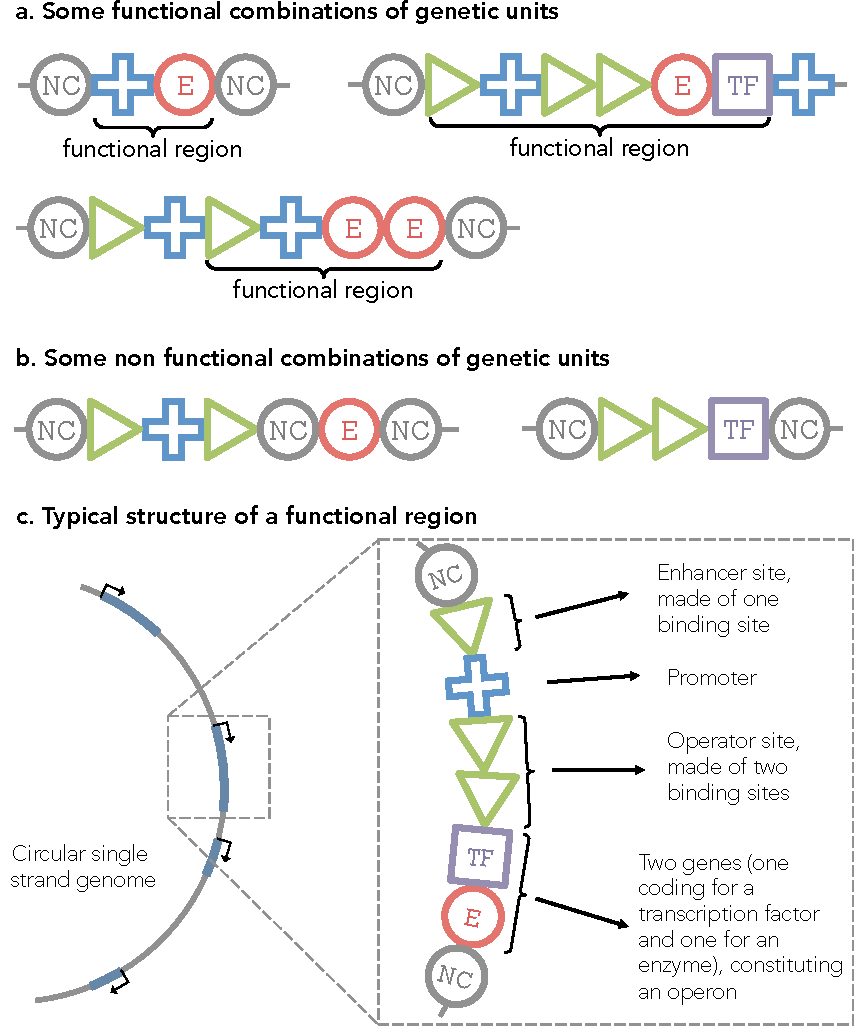
\includegraphics[width=0.8\textwidth]{part2_functional_regions.pdf}
\caption[Some examples of arrangements of genetic units forming functional or non-functional regions.]{\textbf{Some examples of arrangements of genetic units forming or non-functional functional regions.} Grey circles: non-coding units (\textbf{NC}). Blue triangles: binding site units (\textbf{BS}). Orange crosses: promoter units (\textbf{P}). Purple squares: transcription factor coding units (\textbf{TF}). Magenta circles: enzyme coding units (\textbf{E}). The functional regions of a genome are those that have the following pattern: a promoter (\textbf{P}), optionally flanked upstream (enhancer site) or downstream (operator site) by one or more binding sites (\textbf{BS}), followed by one or more contiguous coding units (\textbf{E} or \textbf{TF}). \textbf{a.} Some functional combinations of genetic units. \textbf{b.} Some non functional combinations of genetic units. \textbf{c.} An example of the structure of a typical functional region. The genome is a circular single-strand genome with a single reading frame. A zoom is done in one functional region (magenta regions). The rest of the genome (in grey) is non-coding (non-coding units or any type of unit not correctly arranged to form a functional region).}
\label{fig:part2:methodology:functional_regions}
\end{figure}

%%%%%%%%%%%%%

\subsection{Mutational operators}
\label{subsec:part2:methodology:mutational_operators}

At each replication, the genome undergoes \textbf{point mutations} and \textbf{large rearrangements} (duplications, deletions, translocations and inversions). To account for the effects of these events on the coarse-grained genome, two additional types of mutation have been introduced in {\EvoEvoSim}: \textbf{(i)} \textbf{transitions} : a genetic unit can transit from one type to any other at a certain rate, and \textbf{(ii)} \textbf{breakpoints}: during large rearrangements, genetic units located on sequence breakpoints are exposed to mutations.

\begin{enumerate}
\item[\textbf{(1)}] \textbf{Point mutations.} Point mutations modify the attributes of a genetic unit by adding random values to them. Each attribute (see Table~\ref{table:part2:genetic_units}) owns a dedicated \textbf{mutation kernel} whose properties are predefined as model parameters (usually uniform or gaussian). Two types of attribute exist: integer values and floating-point values. Integer variables mutate by adding a random value from a uniform distribution. Floating-point variables mutate by adding a random value from a normal distribution. For example, the basal expression level $\beta$ (a floating-point variable) mutation kernel is a normal law with a variance defined by the user at the beginning of the simulation. The substrate tag $s$ (an integer value) mutation kernel is a uniform law with a range defined by the user at the beginning of the simulation. In summary, the parameters of eight mutation kernels have to be set by the user (see the {\EvoEvoSim} user guide in Appendix \ref{ch:appendix:user_manual}). Besides the parametrization of the mutation kernels, the \textbf{point mutation rate} must be set by the user. The point mutation rate is expressed per attribute per replication;
\item[\textbf{(2)}] \textbf{Transitions.} Genetic units can also undergo a type transition from any unit type to any other at a rate defined by the user. The transition rate is expressed per genetic unit per replication. All types of genetic units are actually implemented as a tuple containing all possible attributes, like $(\text{unit\_type}, \beta, s, p, k_{cat}, k_{cat}/K_M)$. The unit type tells us which parameters are functionally relevant and the others are free to mutate neutrally. Doing so, digital organisms can explore the neutral fitness landscape and potentially innovate if a non-coding unit is re-functionalized by a type transition (as it the case for pseudogenes);
\item[\textbf{(3)}] \textbf{Duplications.} Large duplications consist in duplicating a random sequence on the genome, and inserting the duplicate at a random location. To select the random sequence to duplicate, two random locations are uniformly drawn in the whole genome. The insertion point is also drawn uniformly (for example, it is possible to insert a duplicate in the duplicated sequence). A duplication implies one breakpoint (Fig. \ref{fig:part2:methodology:large_rearrangements}a). The duplication rate is expressed per genetic unit per replication;
\item[\textbf{(3)}] \textbf{Deletions.} Large deletions consist in deleting a random sequence from the genome, and join the two extremities of the remaining sequence. To select the random sequence to delete, two random locations are uniformly drawn. A deletion implies two breakpoints (Fig. \ref{fig:part2:methodology:large_rearrangements}b). The deletion rate is expressed per genetic unit per replication;
\item[\textbf{(4)}] \textbf{Translocations.} Large translocations consist in moving a random sequence from one genome location to another. To select the random sequence to move, two random locations are uniformly drawn. The insertion point is also drawn uniformly in the whole genome. A translocation implies three breakpoints (Fig. \ref{fig:part2:methodology:large_rearrangements}c). The translocation rate is expressed per genetic unit per replication;
\item[\textbf{(5)}] \textbf{Inversions.} Large inversions consist in reverting a random sequence on the genome. To select the random sequence to revert, two random locations are uniformly drawn in the whole genome. An inversion implies two breakpoints (Fig. \ref{fig:part2:methodology:large_rearrangements}d). The inversion rate is expressed per genetic unit per replication;
\item[\textbf{(6)}] \textbf{Breakpoints.} In real genomes, spontaneous rearrangement breakpoints have no reason to lie exactly between two functional regions and could thus break them. To model that with the coarse-grained genome representation, the content of the two genetic units that are adjacent to a rearrangement breakpoint is altered. Suppose for example that a deletion joins two genetic units, one containing the attributes ($\text{unit\_type}_1$, $\beta_1$, $s_1$, $p_1$, $k_{cat1}$, $(k_{cat}/K_M)_1$) and the other the attributes ($\text{unit\_type}_2$, $\beta_2$, $s_2$, $p_2$, $k_{cat2}$, $(k_{cat}/K_M)_2$). Then for each attribute, there is a probability for the value in unit 1 to be exchanged with the value in unit 2. Both units could for example exchange their values of $s$, thereby leading to ($\text{unit\_type}_1$, $\beta_1$, $s_2$, $p_1$, $k_{cat1}$, $(k_{cat}/K_M)_1$) and ($\text{unit\_type}_2$, $\beta_2$, $s_1$, $p_2$, $k_{cat2}$, $(k_{cat}/K_M)_2$). The breakpoint rate is expressed per breakpoint per replication, and must be set by the user.
\end{enumerate}

\begin{figure}[!h]
\centering 
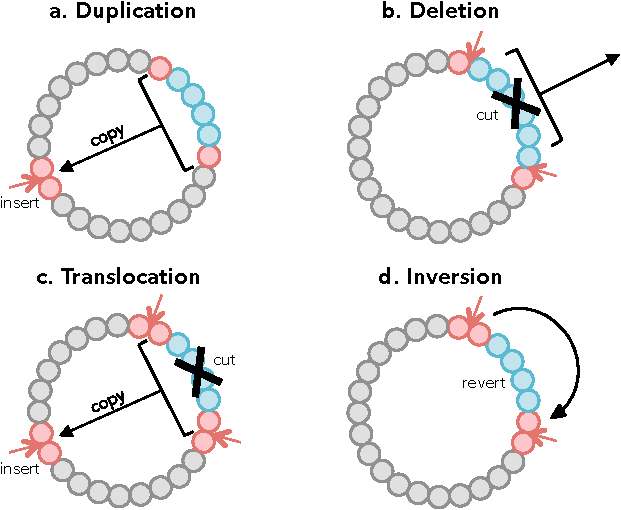
\includegraphics[width=0.8\textwidth]{part2_large_rearrangements.pdf}
\caption[The four types of large rearrangements in {\EvoEvoSim}.]{\textbf{The four types of large rearrangements in {\EvoEvoSim}.} At replication, genomes undergo four types of large rearrangements: \textbf{a.} duplications, \textbf{b.} deletions, \textbf{c.} translocations, and \textbf{d.} inversions. The genome sequence targeted by the rearrangement is colored in blue. Breakpoints are represented by red arrows. The genetic units undergoing mutations at breakpoints are colored in red.}
\label{fig:part2:methodology:large_rearrangements}
\end{figure}

%%%%%%%%%%%%%%%%%%%%%%%%% SECTION : THE GENETIC REGULATORY NETWORK %

\section{The genetic regulatory network}
\label{sec:part2:methodology:grn}

When transcription factors are expressed, they can contribute to the genetic regulatory network by binding to functional enhancer or operator sites. At each time-step $t$ and for each promoter $i$ belonging to a functional region, four steps are necessary to compute the activity of the network:

\begin{enumerate}

% COMPUTE BINDING SITE ACTIVITY
\item[\textbf{(1)}] The activity $A_s(t)$ of each binding site $s$ reads:

\begin{equation}
\label{eq:part2:methodology:binding_site_activity}
A_s(t) = \sum_j c_j(t) A_{js}
\end{equation}

with $c_j(t)$ the concentration of the transcription factor $j$ at time $t$ and $A_{js} \in [0, 1]$ the affinity of this transcription factor for the binding site $s$. In the following, all the concentrations will be expressed in \textbf{arbitrary concentration units} (ACU).
The affinity $A_{js}$ depends on the distance between the transcription factor tag $\text{TF}_\text{tag}(j) \in \mathbb{Z}$ and the binding site tag $\text{BS}_\text{tag}(j) \in \mathbb{Z}$, and the binding window $W_\text{bind}(j)$ of the transcription factor $j$. It reads:

\begin{equation}
\label{eq:part2:methodology:affinity}
A_{js} = \left\{
\begin{array}{l l}
1-\dfrac{|\text{TF}_\text{tag}(j) - \text{BS}_\text{tag}(j)|}{W_\text{bind}(j)} & \text{if \quad $|\text{TF}_\text{tag}(j) - \text{BS}_\text{tag}(j)| \leq W_\text{bind}(j)$}\\\\
0 & \text{else}
\end{array}
\right.
\end{equation}

Figure \ref{fig:part2:methodology:affinity} shows the variation of the affinity when the distance between the transcription factor tag and the binding site tag varies.

\begin{figure}[!ht]
\centering 
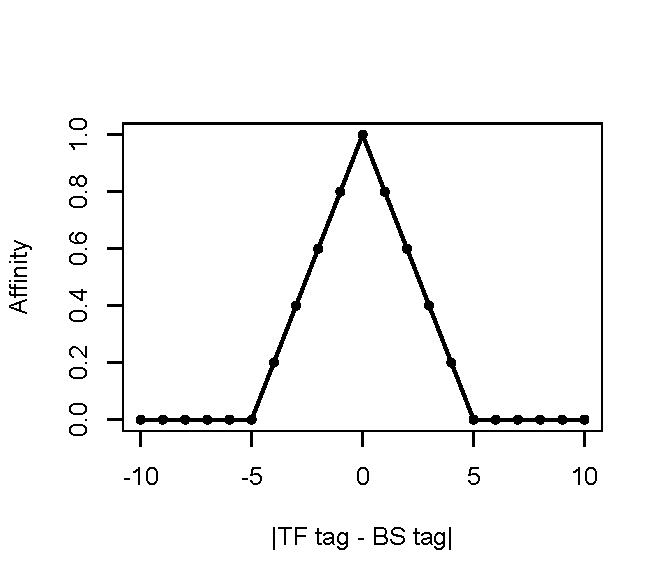
\includegraphics[width=0.5\textwidth]{part2_affinity.pdf}
\caption[The affinity of a transcription factor for a binding site depends on the distance between their respective tags.]{\textbf{The affinity of a transcription factor for a binding site depends on the distance between their respective tags.} On x-axis, the distance between the transcription factor tag and the binding site tag. On y-axis, the affinity computed thanks to Eq~\ref{eq:part2:methodology:affinity}. Here the binding window $W_\text{bind} = 5$.}
\label{fig:part2:methodology:affinity}
\end{figure}

% COMPUTE ENHANCER AND OPERATOR REGIONS ACTIVITY
\item[\textbf{(2)}] From \textbf{(1)}, the activities of the enhancer site $E_i(t) > 0$ and of the operator site $O_i(t) > 0$ flanking the promoter $i$ read:

\begin{equation}
\label{eq:part2:methodology:enhancer_operator_activity}
\left\{
\begin{array}{rcl}
E_i(t) & = & \sum\limits_{s\ \in\ \text{enhancer}_i} A_s(t)\\\\
O_i(t) & = & \sum\limits_{s\ \in\ \text{operator}_i} A_s(t)
\end{array}
\right.
\end{equation}

% COMPUTE THE EXPRESSION RATE
\item[\textbf{(3)}] Then, the expression rate $e_i(t)$ of the promoter $i$ is given by the following Hill-like function:

\begin{equation}
\label{eq:part2:methodology:hill_function}
e_i(t) = \beta_i . \left( \dfrac{\theta^n}{O_i(t)^n + \theta^n} \right) . \left( 1 + \left( \dfrac{1}{\beta_i} - 1 \right) . \left( \dfrac{E_i(t)^n}{E_i(t)^n + \theta^n} \right) \right)
\end{equation}

with $\beta_i \in [0, 1]$ the basal expression level of the promoter $i$, $n$ and $\theta$ two constants shaping the Hill-like function (defined by the user).

% COMPUTE THE EVOLUTION OF PROTEIN CONCENTRATIONS
\item[\textbf{(4)}] At each time-step $t$, coding units being controlled by the promoter $i$ are expressed at a rate $e_i(t)$. Then, the concentration of each protein depending on the promoter $i$ in the cytoplasm depends on the following synthesis-degradation rule:

\begin{equation}
\left\{
\begin{array}{l}
c_i(0) = \dfrac{\beta_i}{\phi}\\\\
\dfrac{\partial c_i}{\partial t} = e_i(t) - \phi . c_i(t)
\end{array}
\right.
\end{equation}

with $\phi$ the protein degradation rate, set by the user before the beginning of any simulation.

\end{enumerate}

%%%%%%%%%%%%%%%%%%%%%%%%% SECTION : THE METABOLIC NETWORK %

\section{The metabolic network}
\label{sec:part2:methodology:metabolism}

Enzyme coding units products can either be pumps, pumping metabolites from or to the growth medium, or enzymes performing catalytic transformations in the metabolic space.
 
Let us consider an enzyme in the cytoplasm that catalyzes one specific reaction $s \rightarrow p$ (with $s \in \mathbb{N}^*$ and $p \in \mathbb{N}^*$ being the substrate and the product of a Michaelis-Menten-like reaction, respectively). The variation in concentrations $[s]$ and $[p]$ over time are then driven by Eq~\ref{eq:michaelis_menten}:

\begin{eqnarray}
\label{eq:michaelis_menten}
\left\{
\begin{array}{lcr}
\dfrac{d[s]}{dt} = -\dfrac{k_{cat}[E][s]}{K_M+[s]}\\\\
\dfrac{d[p]}{dt} = \dfrac{k_{cat}[E][s]}{K_M+[s]}
\end{array}
\right.
\end{eqnarray}

where $K_M$ and $k_{cat}$ are the kinetic attributes of the enzyme ($K_M$ being deduced from $k_{cat}$ and $k_{cat}/K_M$ attributes).

Is $s=p$, enzymes are treated as pumps, for which $[s]$ and $[p]$ describe the internal and external concentrations of the same metabolite. If $k_{cat}$ is positive (resp. negative), $[s]$ is the external (resp. internal) concentration of the metabolite and $[p]$ the internal (resp. external) concentration. The dynamics of metabolic concentrations $[s]$ and $[p]$ are thus also driven by Eq~\ref{eq:michaelis_menten} when the enzyme coding unit product is a pump.

%%%%%%%%%%%%%%%%%%%%%%%%% SECTION : COUPLING NETWORKS %

\section{Coupling the genetic regulatory network and the metabolic network}
\label{sec:part2:methodology:coupling_networks}

Bacteria are able to sense their environment by detecting the presence of a particular molecule or signal, and to give an appropriate answer by updating their gene expression profile. The archetype of this behaviour is the \textbf{lactose operon} \citep{jacob-and-monod-1961}.

As shown in Figure \ref{fig:part2:methodology:lactose_operon}, this operon is composed of three genes (\textit{lacZ}, \textit{lacY} and \textit{lacA}), controlled by one promoter flanked by an operator. Another gene, \textit{lacI}, codes for a transcription factor which inhibates the operon when binding on the operator. \textit{lacI} is constitutively expressed and its concentration in the cytoplasm is almost constant. However its conformation, hence its affinity for the operator is modified by lactose. In absence of lactose, \textit{lacI} is active and down-regulates the operon. If lactose is present, it binds on \textit{lacI} and inhibits it. In this case, the operon is expressed and the cell is able to degrade lactose.

This mechanism is integrated to {\EvoEvoSim}: some metabolites can behave as co-enzymes, and repress or activate transcription factors activity. To this aim, each transcription factor own a co-enzyme tag $\text{CoE}_\text{tag} \in \mathbb{N}^*$, a co-enzyme constant $k_\text{CoE}$, a free activity $A_{\text{free}}$ and a bound activity $A_{\text{bound}}$. A metabolite $m$ can repress or activate a transcription factor in four ways:
\begin{enumerate}
\item[\textbf{(1)}] If $A_{\text{free}} = 1$ and $A_{\text{bound}} = 0$, $m$ inhibits the transcription factor;
\item[\textbf{(2)}] If $A_{\text{free}} = 0$ and $A_{\text{bound}} = 1$, $m$ activates the transcription factor;
\item[\textbf{(3)}] If $A_{\text{free}} = 1$ and $A_{\text{bound}} = 1$, the transcription factor is always activated;
\item[\textbf{(4)}] If $A_{\text{free}} = 0$ and $A_{\text{bound}} = 0$, the transcription factor is always repressed.
\end{enumerate}

\begin{figure}[!h]
\centering 
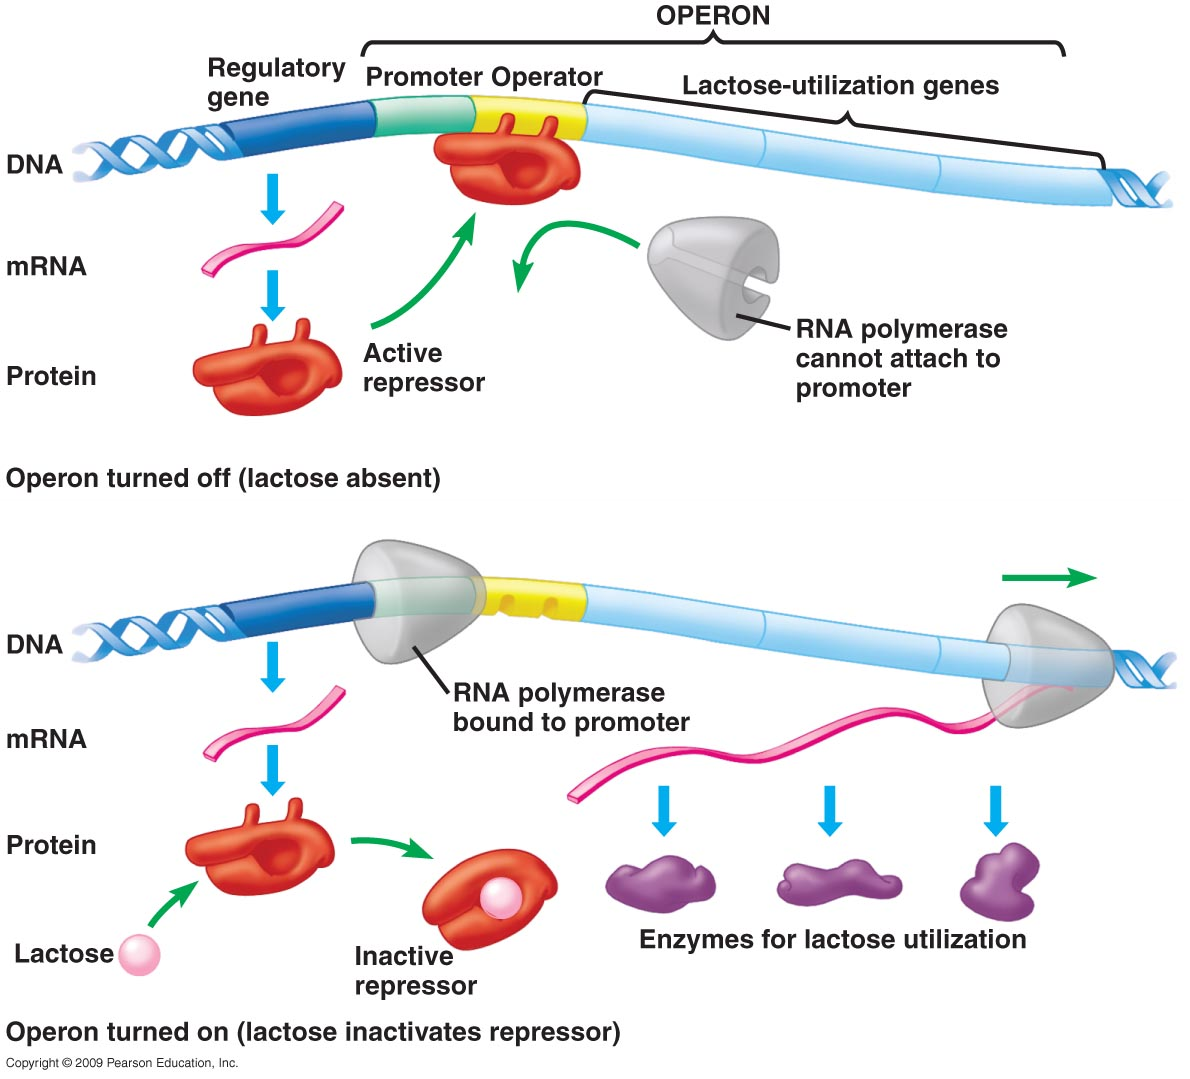
\includegraphics[width=0.8\textwidth]{part2_lactose_operon.jpg}
\caption[The lactose operon.]{\textbf{The lactose operon.} The lactose operon is inactive in the absence of lactose (top) because a repressor blocks attachment of RNA polymerase to the promoter. With lactose present (bottom), the repressor is inactivated, and transcription of lactose-processing genes proceeds (from \href{https://2fsfox.blogspot.fr/2013/05/the-lac-operon-continued-and-other.html}{https://2fsfox.blogspot.fr/2013/05/the-lac-operon-continued-and-other.html}).}
\label{fig:part2:methodology:lactose_operon}
\end{figure}

Table~\ref{table:part2:co_enzyme_activity} resumes these different outcomes by using the following picture: let's consider a transcription factor as a structure with two arms, linked by a pivotal point. The active site of the transcription factor is located on one arm, its exposure depending on the equilibrium state (or conformation) of the structure. Two configurations are possible: one when the transcription factor is free, and another when a co-enzyme binds to it via the anchoring points located at arms end. The combination of free and bound activities then leads to four behaviors, as described in Equation \ref{eq:part2:methodology:co_enzyme_activity}.

\begin{equation}
[\text{TF}_+] = 
\left\{
\begin{array}{ccl}
\left[\text{TF}\right] \times \dfrac{k_\text{CoE}}{k_\text{CoE}+[m]} & \text{ if } & A_{free}=1 \text{ and } A_{bound}=0\\\\
\left[\text{TF}\right] \times \dfrac{[m]}{k_\text{CoE}+[m]} & \text{ if } & A_{free}=0 \text{ and } A_{bound}=1\\\\
\left[\text{TF}\right] & \text{ if } & A_{free}=1 \text{ and } A_{bound}=1\\\\
0.0 & \text{ if } & A_{free}=0 \text{ and } A_{bound}=0
\end{array}
\right.
\label{eq:part2:methodology:co_enzyme_activity}
\end{equation}


\begin{tablehere}
\begin{adjustwidth}{0in}{0in}
\centering
\caption[The eight possible states of a transcription factor.]{\textbf{The eight possible states of a transcription factor.} The transcription factor is represented in dark grey. Its active site (the part allowing binding on a binding site) is represented in green. Depending on free and bound activities attributes, the co-enzyme (in blue) acts as an activator or a repressor. The active site is then free (or not) to bind on a binding site.}
\begin{tabular}{ | c | c | c | c |}
\hline
\textbf{Free TF} & \textbf{Bound TF} & \textbf{Free activity} & \textbf{Bound activity}\\
\hline

\begin{minipage}{3cm}
\centering

\includegraphics{TF1.pdf}
\end{minipage}
& 
\begin{minipage}{3cm}
\centering

\includegraphics{TF2.pdf}
\end{minipage}
&
\textit{1}
&
\textit{0}
\\
\hline

\begin{minipage}{3cm}
\centering

\includegraphics{TF3.pdf}
\end{minipage}
& 
\begin{minipage}{3cm}
\centering

\includegraphics{TF4.pdf}
\end{minipage}
&
\textit{0}
&
\textit{1}
\\
\hline

\begin{minipage}{3cm}
\centering

\includegraphics{TF5.pdf}
\end{minipage}
& 
\begin{minipage}{3cm}
\centering

\includegraphics{TF6.pdf}
\end{minipage}
&
\textit{1}
&
\textit{1}
\\
\hline

\begin{minipage}{3cm}
\centering

\includegraphics{TF7.pdf}
\end{minipage}
& 
\begin{minipage}{3cm}
\centering

\includegraphics{TF8.pdf}
\end{minipage}
&
\textit{0}
&
\textit{0}
\\
\hline

\end{tabular}
\begin{flushleft}

\end{flushleft}
\label{table:part2:co_enzyme_activity}
\end{adjustwidth}
\end{tablehere}




%%%%%%%%%%%%%%%%%%%%%%%%% SECTION : ENERGY CONSTRAINTS %

\section{Optional feature: energy constraints}
\label{sec:part2:methodology:energy_constraints}

One of the most evident constraints living organisms must cope with in the real world are the laws of thermodynamics. Indeed, real organisms cannot violate the energy balance with their environment, or have negative entropy. One direct consequence is that global entropy cannot decrease, whatever the organism's activity. For example, catabolic reactions produce heat, that will propagate in the local environment of the organism (and possibly kill it). This energy is lost for the organism.
In this sense, life could be seen as a fight against entropy \citep{alberts-et-al-2013}, as illustrated in Figure \ref{fig:part2:methodology:desk_entropy}.
Billions years of evolution made cells very efficient engines to exploit the energy gained with catabolism. Energy carriers, like ATP molecules, allow cells to transfer the energy won by degrading food, or capturing photons, in useful but costly reactions (for example, producing---or actively degrading---a protein). This coupling between food process (catabolism), and production of useful macromolecules (anabolism) is at the heart of cell's metabolism.

We introduced energy constraints in {\EvoEvoSim} by doing the distinction between two types of reactions: reactions rewarding the cell in energy (catabolic reactions), and reactions consuming energy (anabolic reactions). Implicit energy carrier molecules allow us to compute the \textbf{energy balance} $\mathcal{E}$ of the cell at each time-step $t$. To this aim, we introduced a notion of reaction cost, each type of reaction owning a specific cost defined by the user before the beginning of a simulation. There are four energy costs:
\begin{enumerate}
\item[\textbf{(1)}] The \textbf{expression cost} $c_{\text{expr}} \geq 0$: the cell consumes energy when proteins are expressed;
\item[\textbf{(2)}] The \textbf{degradation cost} $c_{\text{degr}} \geq 0$: the cell consumes energy when proteins are degraded (symbolizing, \textit{e.g.}, the functioning of the proteasome);
\item[\textbf{(3)}] The \textbf{enzymatic cost} $c_{\text{enz}} \geq 0$: depending on the type of metabolic reaction (see below), the cell consumes or produces energy when an enzymatic reaction is performed;
\item[\textbf{(4)}] The \textbf{pumping cost} $c_{\text{pump}} \geq 0$: the cell consumes energy when a metabolite is pumped in or out;
\end{enumerate}

\begin{figure}[!h]
\centering 
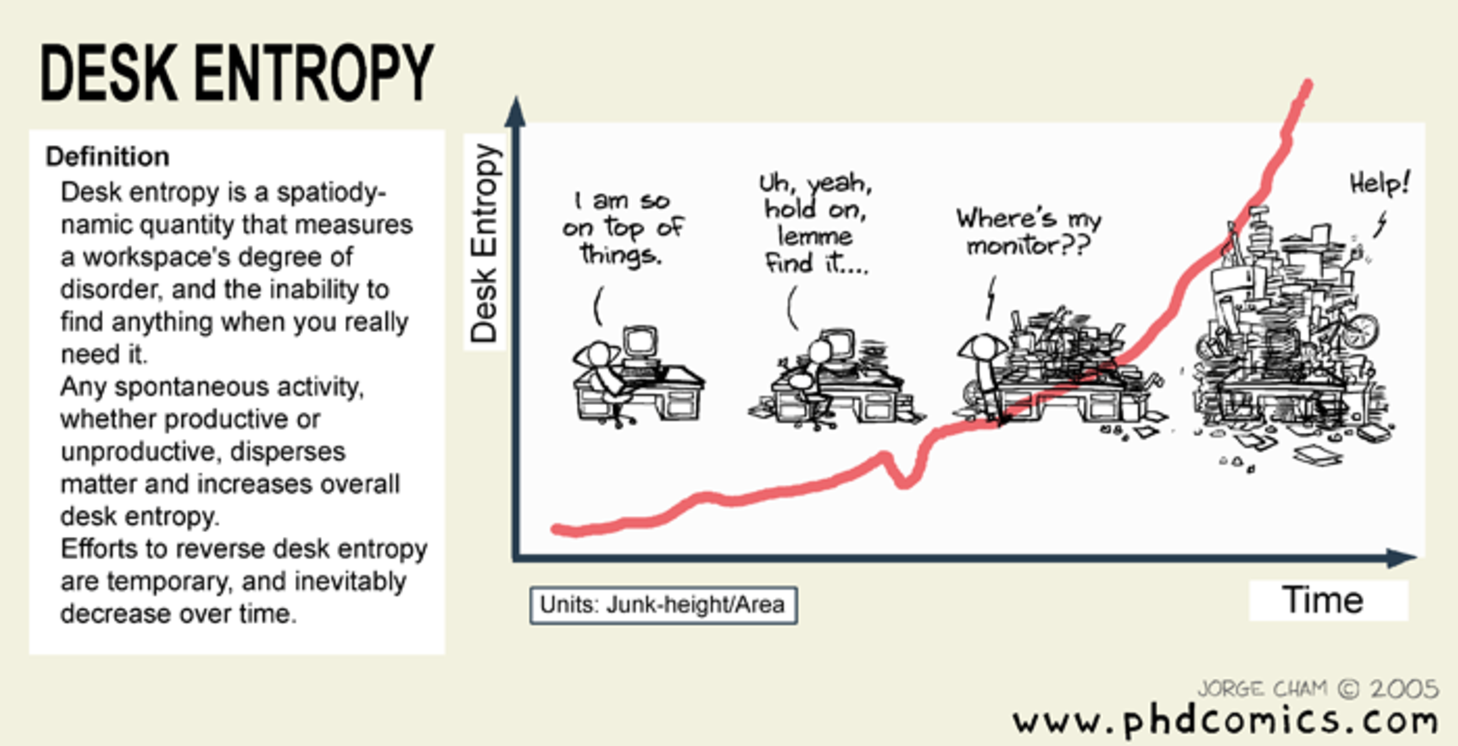
\includegraphics[width=1\textwidth]{part2_deskentropy.pdf}
\caption[An impossible-to-win fight against entropy.]{\textbf{An impossible-to-win fight against entropy.} An illustration of the unavoidable increase of entropy in a system (from \href{www.phdcomics.com}{www.phdcomics.com}).}
\label{fig:part2:methodology:desk_entropy}
\end{figure}

Enzymatic reactions consume or produce energy depending on the values of the substrate tag $s$, the product tag $p$ and the enzymatic cost $c_{\text{enz}}$:
\begin{enumerate}
\item[\textbf{(1)}] if $s < p$, the reaction consumes energy at a rate $(p-s) . c_{\text{enz}}$
\item[\textbf{(2)}] if $s > p$, the reaction produces energy at a rate $(s-p) . c_{\text{enz}}$
\end{enumerate}

It is then possible to describe the evolution of the energy balance $\mathcal{E}$ through time, as following:

\begin{equation}
\label{eq:part2:methodology:energy_balance}
\left.
\begin{array}{rcl}
\dfrac{\partial \mathcal{E}}{\partial t} & = & \sum\limits_{i\ \in\ \text{catabolic reactions}} \left( \dfrac{\partial [p_i]}{\partial t} \times (s_i - p_i) \times c_{\text{enz}} \right)\\\\
& - & \sum\limits_{i\ \in\ \text{anabolic reactions}} \left( \dfrac{\partial [p_i]}{\partial t} \times (p_i - s_i) \times c_{\text{enz}} \right)\\\\
& - & \sum\limits_{i\ \in\ \text{inflowing pumps}} \left( \dfrac{\partial [s_{in}]}{\partial t} \times (s_{in} - s_{out}) \times c_{\text{pump}} \right)\\\\
& - & \sum\limits_{i\ \in\ \text{outflowing pumps}} \left( \dfrac{\partial [s_{out}]}{\partial t} \times (s_{out} - s_{in}) \times c_{\text{pump}} \right)\\\\
& - & \sum\limits_{i\ \in\ \text{expressed genes}} \left( \dfrac{\partial [e_i]}{\partial t} \times c_{\text{expr}} \right)\\\\
& - & \sum\limits_{i\ \in\ \text{degraded proteins}} \left( [c_i] \times \phi \times c_{\text{degr}} \right)
\end{array}
\right.
\end{equation}

For practical reasons, $\mathcal{E}$ is not solved as an ordinary differential equation. Indeed, incorporating energy in differential equations would have lead to intractable simulations. For this reason, the energy balance $\mathcal{E}$ is evaluated at the end of each simulation time-step $t$. The cell's score is impaired if the energy balance $\mathcal{E} \leq 0$ (the score function is described below).

%%%%%%%%%%%%%%%%%%%%%%%%% SECTION : THE SCORE FUNCTION %

\section{The score function}
\label{sec:part2:methodology:score_function}

The set of all metabolites contained in the cell's cytoplasm can be converted into a unique concentration vector $\boldsymbol{M} = \{m_1, m_2, ..., m_n\}$. In {\EvoEvoSim}, $\boldsymbol{M}$ constitutes the ``phenotype'' determining the score $S$ of the cell. It is then possible to define a score function $f : \mathbb{R}^n \rightarrow \mathbb{R}_+$ such that $S = f(\boldsymbol{M})$.

Some metabolites are essential to cell's growth, and some other are intermediate products or waste. In {\EvoEvoSim}, essential metabolites are \textbf{prime numbers}: their production contributes to the growth rate by increasing the probability to produce offspring. However, producing metabolites above a predefined threshold leads to cell's toxicity, and impairs cell's score. Let's define the subset of $\boldsymbol{M}$ representing the essential metabolites $\boldsymbol{E} = \{e_1, e_2, ..., e_m\} \subset \boldsymbol{M}$. Then, the score $S$ of the cell is:
\begin{equation}
S = 
\left\{
\begin{array}{lcr}
\sum_i e_i & \mbox{if} & (\forall e \in \boldsymbol{E}\  |\ e < T_E) \cup  (\forall m \in (\boldsymbol{M} \backslash \boldsymbol{E})\  |\ m < T_M)\\\\
0 & \mbox{else} &
\end{array}
\right.
\end{equation}
with $T_M$ the toxicity threshold of non-essential metabolites ($\boldsymbol{M} \backslash \boldsymbol{E})$ and $T_E$ the toxicity threshold of essential metabolites ($\boldsymbol{E}$).

If the cell's score is under a minimum score $S < S_{\text{min}}$ defined by the user, then $S = 0$.

Importantly, the score and the fitness are different. The score represents the instantaneous performance of a cell (being computed at each time-step), while the fitness is usually defined as the combined effect of survival and reproduction, and can only be computed \textit{a posteriori}, when the whole cell's history is known. We will never compute the fitness in {\EvoEvoSim}. Instead, we will analyze the lineage of the final population, that is supposed to have increased its mean fitness through time, in order to recover evolutionary events.

%%%%%%%%%%%%%%%%%%%%%%%%% SECTION : POPULATION AND SELECTION %

\section{Population and selection}
\label{sec:part2:methodology:population_selection}

Organisms evolve on a two-dimensional toroidal grid (each location containing at most one organism), and compete for the external metabolites to produce offspring in empty locations. They interact with their local environment by pumping metabolites in and out and they release their metabolic content at death. At each time-step, organisms are evaluated and either killed, updated or replicated depending on their current state:
\begin{enumerate}
\item[\textbf{(1)}] If the organism does not die and cannot divide (\textit{e.g.}, because there is no free space in its neighborhood), its metabolic network is updated, and its score is computed;
\item[\textbf{(2)}] Organisms can also die randomly with a probability following a Poisson law of parameter $p_{death}$ expressed per organism per time-step. At death, the metabolic content of a cell is released into the local environment;
\item[\textbf{(3)}] For each empty grid location, all living organisms in the Moore neighborhood whose score is higher than a minimum score $S_{min}$ compete. The organism having the best score in the neighborhood is allowed to divide if it did not replicate previously at the same time-step (such that any dividing cell generates at most two daughters per time-step).
\end{enumerate}

%%%%%%%%%%%%%%%%%%%%%%%%% SECTION : ENVIRONMENT %

\section{The environment}
\label{sec:part2:methodology:environment}

The physical environment is described at the grid level: each grid location contains external metabolites, each with its concentration.
These external metabolites diffuse with a diffusion parameter $D$ expressed in gridstep\textsuperscript{2}.time-step\textsuperscript{-1}, meaning that a fraction $D$ of each metabolite present at one location will diffuse to each of the eight neighboring grid locations at each time-step. The discrete diffusion equation we are using is inspired from \cite{frenoy-et-al-2013}. External metabolites are also degraded with a degradation rate $D_g$, meaning that a fraction $D_g$ of each metabolite at each location will disappear at each time-step. We made the simplifying assumption that there are no enzymatic reaction in the environment, and that metabolite transformation only occurs inside the organisms.

At each time-step $t$, each grid location $k$ of coordinates $(x,y)$ is characterized by the individual occupying the location (possibly none), and the list of free metabolites, each metabolite $i$ being at concentration $c_{i,k}(t)$. Given the parameters of the environment, the dynamics of a free metabolite $i$ in a grid location $k$ reads:
\begin{equation}
\label{eq:part2:methodology:environment}
c_{i,k}(t+1) = c_{i,k}(t) - D_g . c_{i,k}(t) + \sum_{j\ \in\ \text{neighbors}} D . c_{i,j}(t) - 8 . D . c_{i,k}(t) + I_i(t)
\end{equation}
With $I_i$ the inflow rate of metabolite $i$ in the environment.

In conclusion, {\EvoEvoSim} allows for a precise parametrization of the environment. Apart from parameters described above, it is possible for the user to set a variety of behaviors (\textit{e.g.} the periodicity of metabolites influx, the type of metabolites provided or their locations, ...). It is thus possible to mimic realistic experimental setups, such as chemostat or batch-culture, as we will discuss in the next chapter.

%%%%%%%%%%%%%%%%%%%%%%%%% SECTION : TROPHIC NETWORKS %

\section{Trophic networks}
\label{sec:part2:methodology:trophic_networks}

Cells uptake various metabolites, provided externally or being by-products released by other cells. {\EvoEvoSim} keeps trace of the metabolic activity of every cells and computes, at each time-step, a \textbf{trophic network} representing the relationships between cells. This feature is mandatory to study, for example, the evolution of cross-feeding in the population. 

At each time-step $t$, a \textbf{trophic profile} is computed for each organism from its metabolic network activity. The trophic profile is a bit string summarizing the uptake, production, and release activity of an organism. The length of the bit string is defined by the largest metabolite tag present in the system at time $t$. For example, if an organism uptakes metabolite $\#4$, produces $\#3$ from $\#4$ and releases $\#3$, knowing that the largest metabolite tag in the system is $\#5$, then its profile is $|00010|00100|00100|$. Organisms with identical trophic profiles are grouped together, and the trophic network is computed depending on profile relationships. For example, if organisms of a profile $i$ uptake a metabolite produced by a profile $j$, then a directed link is created from $i$ to $j$. Cooperating links are also computed: a cell cooperates with another cell if the former \textbf{actively} releases metabolites useful to the latter.

Trophic profiles are then classified in four \textbf{trophic levels}:
\begin{enumerate}
\item[\textbf{(1)}] \textbf{Level 0} cells exclusively feed on exogenous metabolites, flowing in the environment;
\item[\textbf{(2)}] \textbf{Level 1} cells feed on exogenous metabolites and on metabolites produced by other cells;
\item[\textbf{(3)}] \textbf{Level 2} cells exclusively feed on metabolites produced by other cells;
\item[\textbf{(4)}] \textbf{No level} cells have no active uptaking functions.
\end{enumerate}

Figure \ref{fig:part2:methodology:trophic_network} shows a simple example of trophic network computed on the fly during a simulation, and available in {\EvoEvoSim} HTML viewer (see Appendix \ref{ch:appendix:user_manual}). Exogenously provided metabolites are symbolized by a black node (the \texttt{ENV} node), and other trophic profile nodes are colored depending on their level (purple for level 0, blue for level 1, green for level 2 and grey for no level). Trophic links are represented by solid arrows, cooperating links being represented by dashed arrows.

\begin{figurehere}
\centering 
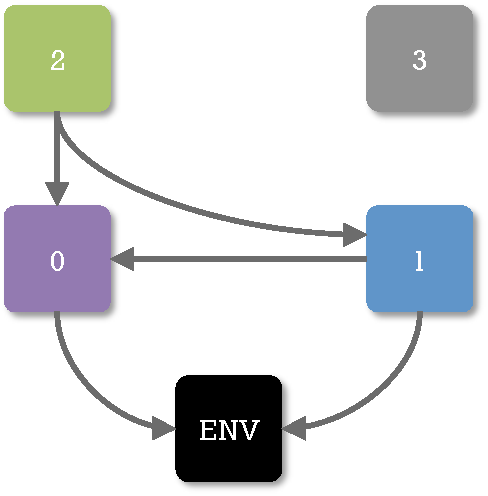
\includegraphics[width=0.3\textwidth]{part2_trophic_network.pdf}
\caption[A basic example of trophic network.]{\textbf{A basic example of trophic network.} A basic example of a trophic network, as it is computed in {\EvoEvoSim}, is presented here. Exogenously provided metabolites are represented by a black node tagged \texttt{ENV}. Trophic profiles (\textit{i.e.}, a group of cells having the exact same metabolic activity) exclusively feeding on exogenous metabolites belong to the level 0, and are represented by purple nodes. Trophic profiles feeding on exogenous metabolites and on by-products of other cells belong to level 1 ; they are represented by blue nodes. Trophic profiles exclusively feeding on by-products are represented by green nodes (level 2). Trophic profiles having no metabolic activity are represented by grey nodes. Here, one level 0 profile feeds on the environment, one level 1 profile feeds on the environment and on profile 0, one level 2 profile feeds on profiles 0 and 1, and one profile has no metabolic activity (no level).}
\label{fig:part2:methodology:trophic_network}
\end{figurehere}

%%%%%%%%%%%%%%%%%%%%%%%%% SECTION : PHYLOGENY %

\begin{figure}[!h]
\centering 
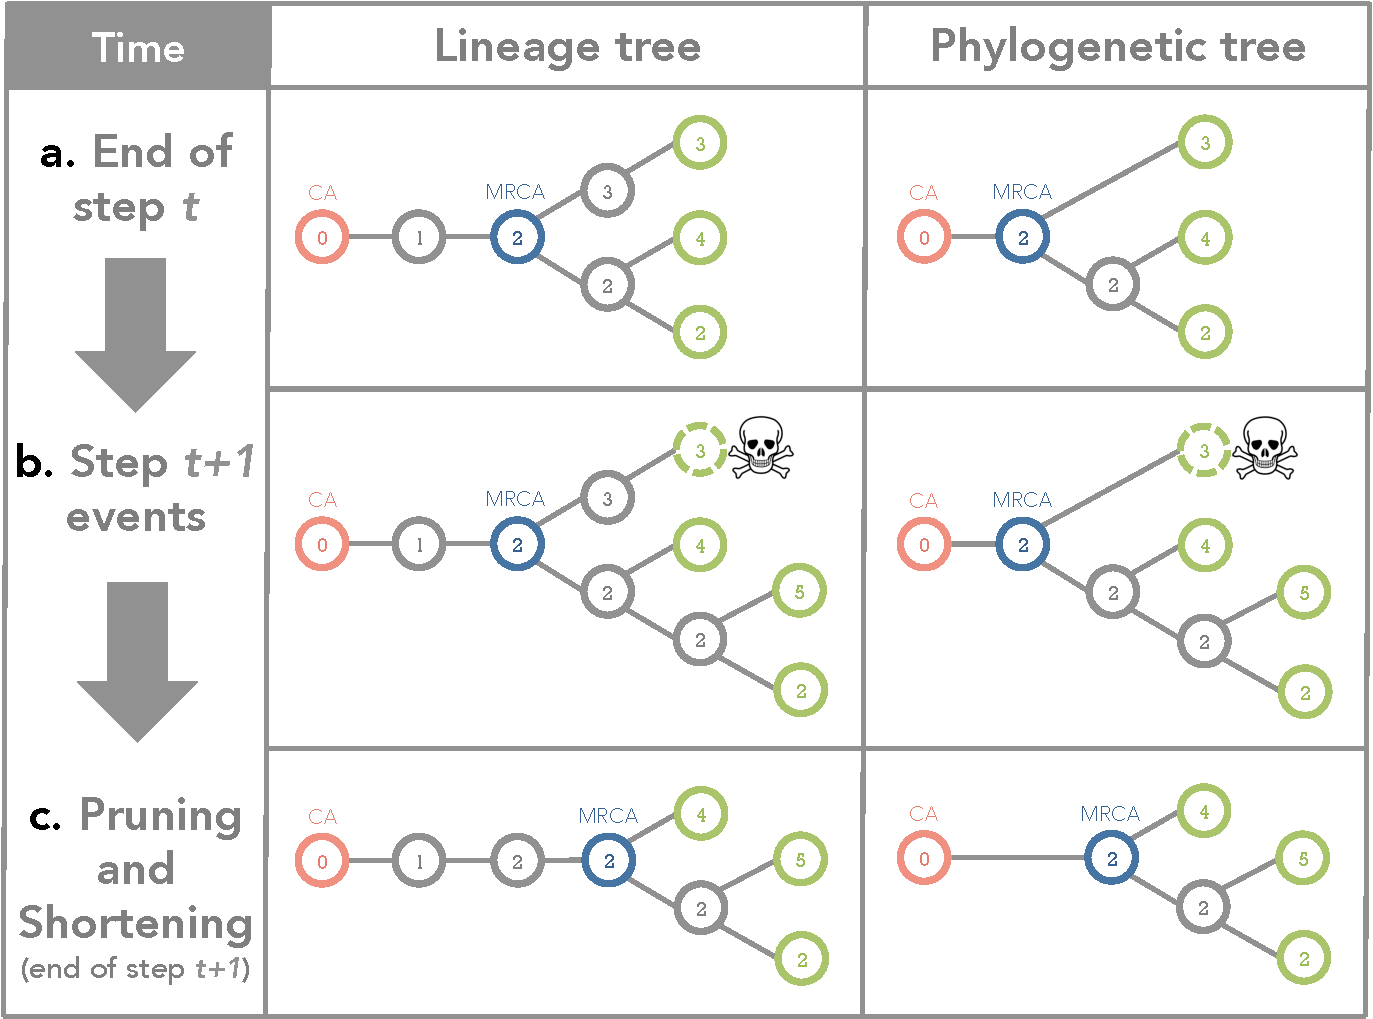
\includegraphics[width=1\textwidth]{part2_trees.pdf}
\caption[Live update of lineage and phylogenetic trees.]{\textbf{Live update of lineage and phylogenetic trees.} At each time-step $t$, the population state is updated (divisions, deaths, cell updates, ...): \textbf{(i)} at each division, the two daughter cells are added to the trees as leaves, with their parent as a common ancestor, \textbf{(ii)} dead cells are removed from trees. Both lineage and phylogenetic trees are pruned (dead branches are removed), and the phylogenetic tree is shortened (intermediate nodes not being common ancestors are removed). \textbf{In this example}, we start at time $t$. The common ancestor of the whole population (\textbf{CA}, in red) is the \textbf{dead cell} labelled $0$. The most recent common ancestor (\textbf{MRCA}, in blue) is the \textbf{alive cell} $2$. Tree leaves are represented in green and all correspond to alive cells (first row). The population state is then updated to time $t+1$: the cell $3$ dies, and the cell $2$ divides in daughter cells $2$ and $5$ (the cell $2$ is still tracked because it divided 4 times and didn't died yet). These events are added to both trees (second row). Then, \textbf{pruning} and \textbf{shortening} algorithms are applied: the lineage tree looses the branch $3-3$. The phylogenetic tree looses the leaf $3$, and the oldest $2$ node. The MRCA is now the node $2$, linked to nodes $2$ and $4$.}
\label{fig:part2:methodology:trees}
\end{figure}

\section{Lineages and phylogeny}
\label{subsec:part2:methodology:phylogeny}

In {\EvoEvoSim}, phylogenetic relationships are exhaustively recorded during a simulation. Two trees are updated at each time-step: the \textbf{lineage tree}, that saves the lineage relationships of every living cells, and the \textbf{phylogenetic tree}, that saves the complete phylogeny of every living cells. Besides phylogenetic relationships, many informations about the genome structure, the phenotype, the mutations, the trophic profile, and so on, are saved in every nodes of the trees. Thus, it is possible to precisely recover the evolution of a population, including fixed mutations. In particular, it is possible to determine if trophic groups are \textbf{monophyletic}, and thus can be considered as \textbf{ecotypes} (see the next chapter for a precise example).

Algorithmically speaking, the phylogenetic tracking deployed in {\EvoEvoSim} is updated as follows: at each simulation time-step $t$, \textbf{(i)} new offspring are added to both trees (Fig. \ref{fig:part2:methodology:trees}b), \textbf{(ii)} both trees are pruned to remove dead branches (Fig. \ref{fig:part2:methodology:trees}c), and \textbf{(iii)} the phylogenetic tree is shortened to remove intermediate nodes between common ancestors (Fig. \ref{fig:part2:methodology:trees}c). One node in the lineage or phylogenetic tree corresponds to one generation in the population. This means that when a cell produces offspring, new nodes are created for the two daughters, even if each cell is individually tracked for its entire life. For example, two or more contiguous nodes in a tree could correspond to a single cell that divided one or more times, as shown in Figure \ref{fig:part2:methodology:trees} with cell $\#2$. In each tree, the common ancestor (CA) of the whole population is tagged (red node on Fig. \ref{fig:part2:methodology:trees}), as well as the most recent common ancestor (MRCA, blue node on Fig. \ref{fig:part2:methodology:trees}).

%%%%%%%%%%%%%%%%%%%%%%%%% SECTION : GENERAL ALGORITHM %

\section{General algorithm}
\label{sec:part2:methodology:general_algorithm}

The general algorithm behind {\EvoEvoSim} is a classical, asynchronous algorithm of \textit{in silico} evolution \citep{hindre-et-al-2012}. At each time-step, each living cell is evaluated, and a decision is made between death, division, or simple update (as presented in Fig.~\ref{fig:part2:methodology:general_algorithm}). The lineage and phylogenetic trees are updated on the fly, as well as the trophic network. In the same time, very complete statistics are computed (tracking hundred of variables), and a large amount of statistics (population means, best individual lineage, phylogeny, ...) are displayed on the fly, in the {\EvoEvoSim} HTML viewer (see Appendix \ref{ch:appendix:user_manual}).

To solve the ordinary differential equations, We used the adaptive Runge-Kutta-Cash-Karp method (RKCK). At each simulation time-step $t$ and for each alive cell, the state of the genetic regulatory network and the metabolic network are updated by solving the ODE system during $t_{\text{ODE}}$ time-steps. This constant is set by the user before the beginning of the simulation (usually $t_{\text{ODE}} = 100$, meaning that each simulation time-step corresponds to 100 ODE time-steps). Altogether, if we consider a $32 \times 32$ environmental grid full of organisms, a time-step involves a thousand of ODE systems. The parameter values of each ODE system are potentially unique, as they are encoded in the organism's genome and thus result from the mutation process. Those ODE systems can also differ by their number of equations, which depends on the organism's genome.

Moreover, {\EvoEvoSim} admits parallel computing algorithms, and is designed for high performance computing (see the user guide in Appendix \ref{ch:appendix:user_manual}).

\newpage
\begin{figurehere}
\centering 
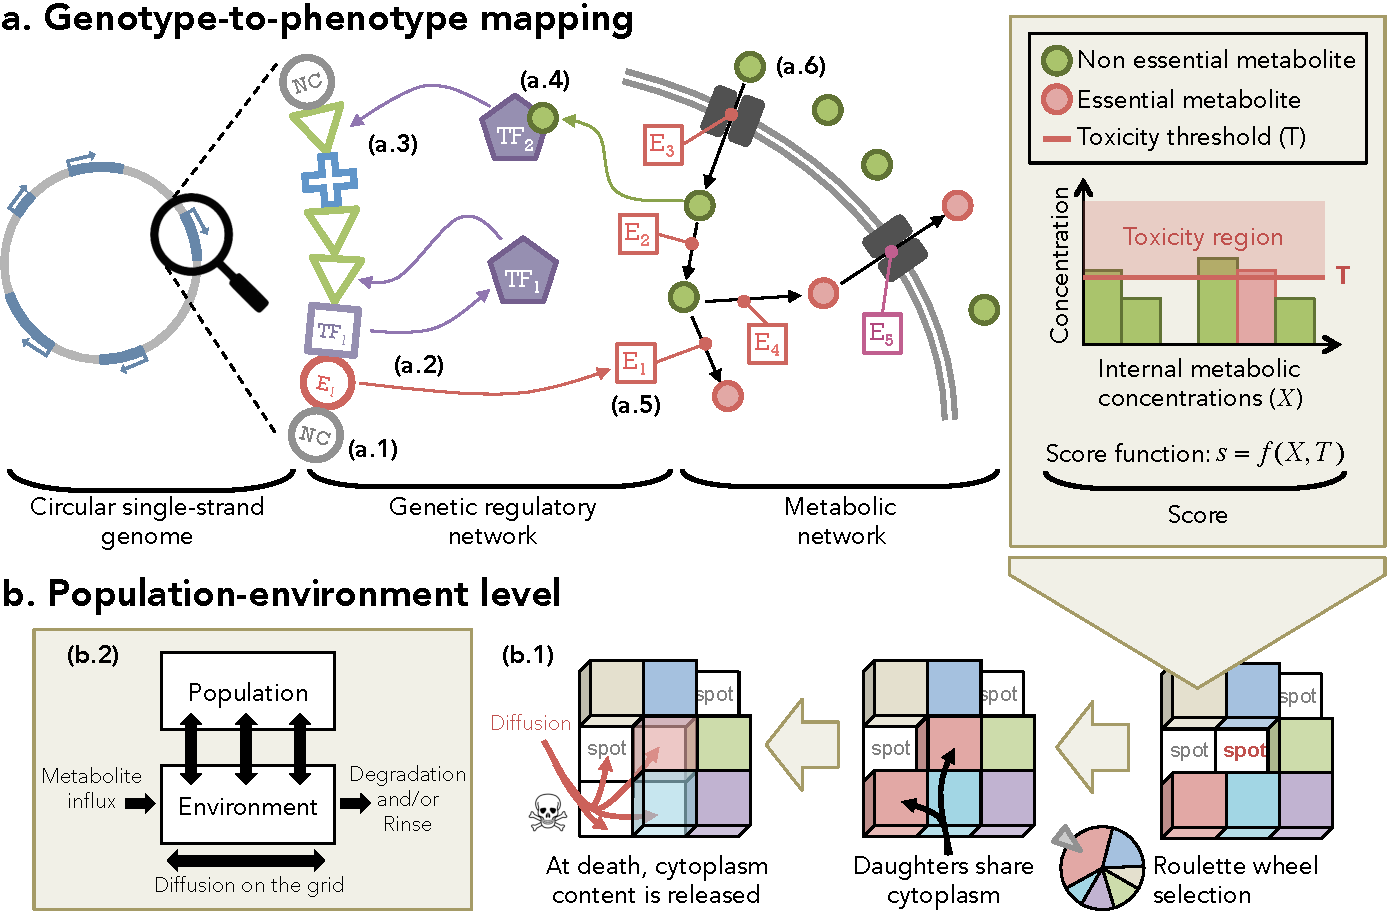
\includegraphics[width=1\textwidth]{part2_general_algorithm.pdf}
\caption[Global picture of {\EvoEvoSim}.]{\textbf{Global picture of {\EvoEvoSim}.} \textbf{a. Description of the genotype-to-phenotype mapping.} Organisms own a coarse-grained genome made of units. This genome is a circular single-strand sequence, with a unique reading frame. Non coding \textbf{(NC)} units are not functional \textbf{(a.1)}. The arrangement of the units on the sequence defines functional regions, where a promoter (\textbf{P}, blue cross) controls the expression of enzyme coding units (\textbf{E}, red circles) or transcription factor coding units (\textbf{TF}, purple squares), thereby allowing for operons (here, one E and one TF). When coding units are expressed \textbf{(a.2)}, they contribute to the genetic regulatory network (for TFs) and the metabolic network (for Es).
Depending on their attributes (see~\ref{sec:part2:methodology:genome} and~\ref{sec:part2:methodology:grn}), transcription factors bind on binding sites. \textbf{(a.3)} If they bind on the enhancer sequence (binding sites flanking the promoter upstream), the promoter activity is up-regulated. If they bind on the operator sequence (binding sites flanking the promoter downstream), the promoter activity is down-regulated. \textbf{(a.4)} Metabolites can bind on a transcription factor as co-enzymes, and activate or inhibit it, depending on transcription factor attributes (see~\ref{sec:part2:methodology:coupling_networks}).
Enzymes perform metabolic reactions in the cytoplasm \textbf{(a.5)}, or pump metabolites in or out \textbf{(a.6)}. The score of an organism is computed from its ``essential metabolites''
(usually the score is the sum of essential metabolite concentrations). Lethal toxicity thresholds are applied to each metabolic concentration and forbid organisms to accumulate resources. \textbf{b. Description of the population and environment levels.} Organisms are placed on a 2D toroidal grid, and compete for resources and space. When an organism dies, it leaves its grid cell empty and organisms in the Moore neighborhood (if any) compete to divide in available space. The competition is based on scores, a minimal threshold being applied on scores to forbid worst organisms to divide. At division, daughters share cytoplasm content (enzymes and metabolites). At death, metabolites from the cytoplasm are released in the local environment, and diffuse on the grid \textbf{(b.1)}. On the largest scale, the population evolves on the environment by up-taking, transforming and releasing metabolites. Metabolites then diffuse and are degraded. This strong interaction between the population and the environment allows for the evolution of complex ecological situations, depending on environmental properties \textbf{(b.2)}.}
\label{fig:part2:methodology:general_algorithm}
\end{figurehere}

%%%%%%%%%%%%%%%%%%%%%%%%% SECTION : CODE AVAILABILITY %

\section{Code availability}
\label{sec:part2:methodology:code_availability}

We developed {\EvoEvoSim} in C++, from scratch. Some scripts are written in Python and R, especially for the automatic generation of live statistics and figures. We also implemented a HTML viewer, including many informations (from best lineage evolution to phylogeny), useful to track evolution during a simulation. This viewer includes some Javascript. The code is hosted on Github in \texttt{charlesrocabert/Evo2Sim} repository. The {\EvoEvoSim} user manual is available in Appendix \ref{ch:appendix:user_manual}. Some simulation examples are also available on the EvoEvo project website at \href{http://evoevo.liris.cnrs.fr/evo2sim/}{http://evoevo.liris.cnrs.fr/evo2sim/}.

%%%%%%%%%%%%%%%%%%%%%%%%% SECTION : WHAT NEXT ? %

\section{What next?}
\label{sec:part2:methodology:what_next}

In the two following chapters, we will present two results obtained with {\EvoEvoSim}. The first has been published in PLoS Computational Biology, and is about niche construction and the evolution of stable cross-feeding. This work does not consider genetic regulation. For this reason, a simplified version of {\EvoEvoSim} will be presented. The second result is preliminary and is about genetic regulation evolution when energy constraints are applied to digital organisms.

